%\documentclass[11pt, twocolumn]{article}
\documentclass[11pt]{article}
\usepackage{multicol}
\usepackage{pslatex}
\usepackage{amsmath}
\usepackage{amssymb}
\usepackage{amsthm}
\usepackage{graphicx}
\usepackage{mathrsfs}
\usepackage{algorithmic}
\usepackage{algorithm}
\usepackage{subfig}
\usepackage{url}
%\usepackage[left=.75in,top=.75in,right=.75in,bottom=.75in]{geometry}
\usepackage[left=1in,top=1.2in,right=1in,bottom=1in]{geometry}

\textwidth 6.5in
\textheight 8.8in

\title{TrackMeNot-so-good-after-all}
\author{Rami Al-Rfou' \\{\texttt{ralrfou@cs.stonybrook.edu}}
\and William Jannen \\{\texttt{wjannen@cs.stonybrook.edu}}
\and Nikhil Patwardhan \\{\texttt{npatwardhan@cs.stonybrook.edu}}
}
\begin{document}

\maketitle

\pagestyle{headings}

\begin{abstract}
  TrackMeNot is a Firefox plugin with laudable intentions - protecting
  your privacy. By issuing a customizable stream of random search
  queries on its users' behalf, TrackMeNot surmises that enough ``search
  noise'' will prevent the users' true query profiles from being
  discerned. However, we find that clustering queries by semantic
  relatedness allows us to disentangle a nontrivial subset of user
  queries from TrackMeNot issued noise.
\end{abstract}
\begin{multicols}{2}
\section{Background}
\label{sec:background}
%Identity theft is a major issue in moern society; as many as 10
%million Americans are victims of identity theft each year
%\cite{spamlaws}. As awareness spreads, the issue of online privacy has
%come into focus as a way to reduce exposure.  

The decreasing cost of persistant media for storage, coupled with the
steady rise in E-commerce, social networking, and various other online
services, has led to a dramatic increase in the volume of readily
available, personally identifiable information. One often overlooked
source of such information is the logging by search engines of user
queries.

There have been several high-profile examples of search query data
being used in inappropriate ways, most notably an incident involving AOL in 2006 \cite{aol}. The company disclosed a data set comprised of  information from 658,000
subscribers' search histories; it was released as a flat file into the public
domain. Upon admitting their error, they removed the link, but the data was already mirrored elsewhere. This incident highlights just how personally revealing search
engine queries can be, as at least one user was identified using only
the content of her searches %\cite{user957}.

The average internet user may browse under the false impression that
deleting cookies or diverting traffic through a proxy will protect
their anonymity on the web. Neither of these measures provide complete
protection. If a user wishes to utilize certain services such as
Google Mail, they must log in to their personal profile. Once logged
in, their queries are then tied to their accout.

TrackMeNot is a Firefox plugin that aims to protect the privacy of its users by issuing random queries on their behalf. These random queries are pulled from a variety of sources, with the intuition that providing enough ``noise'' around a user's true search patterns will make it impossible to disentangle the queries made by TrackMeNot from those actually made by human searchers.

\section{TrackMeNot details}
\label{sec:tmn}
TrackMeNot operates completely on the client side as a Firefox plugin. Upon startup, an initial {\it seed list} is populated from RSS feeds and known public ``popular search'' lists. During execution, queries are pulled from this list and issued to popular search engines on the user's behalf.

The user is offered many parameters, which can be tuned to customize
TrackMeNot behavior. For instance, the user can select which, if any,
popular search engines he wishes TrackMeNot to query on his behalf. If
the user only performs searches at \url{http://www.Google.com}, he can
specify that TrackMeNot query only  that site as well. The user can
also specify the frequency of TrackMeNot queries (the default average
query rate is 10 queries per hour), as well as whether or not to enable {\it query
bursts}. Query bursts are triggered by actual user queries; when
TrackMeNot detects a genuine query, it responds by issuing a batch of
simulated searches. In a subset of query bursts, a longer query is
selected and permuted to form a set of potentially similar searches.

The basis of the TrackMeNot model is its {\it dynamic query
  list}. Starting from the initial seed list, queries are randomly
marked for replacement over time. When a marked query is sent by TrackMeNot as a
search engine request, the HTTP responses are parsed to identify any
suitable ``query-like'' terms for replacement. If an acceptable term
is found, it is then substituted into the dynamic list in exchange for
the marked query. In this way, the list of searches will evolve over
time.

TrackMeNot also attempts to simulate user browsing patterns with
``selective click-through''; upon issuing a random query,
it will parse the results page, using regular expression matching to
identify and remove revenue generating ads. It then selects one or
more of the remaining links on the page and simulates a user click.

Although TrackMeNot simulates temporal search patterns with techniques
like query bursts and selective click-through, it may not sumulate
contextual search patterns - sequential TrackMeNot queries are most
likely semantically unrelated. Individual queries are selected at
random from a 100-200 term dynamic query list. So while it is likely
that the dynamic query list contains related searches, as long as
searches are selected individually at random, there is no guarantee
that related terms will be issued in temporal proximity. This is the
aspect of the TrackMeNot design we wish to exploit.

\section{Design overview}
\label{sec:design}
Our overall design can be logically divided into three parts. The
first part deals with logging all user Google Search queries as well
as those fired from TMN. The second part comprises the computation of
a similarity matrix on this set of queries using a suitable semantic
distance measure. The last part consists of clustering this data using
a suitable technique to get a visual representation of the data from
which conclusions can be deduced.

\section{Data Gathering}

\section{Semantic Distance Measure}
The basic idea here was to find how \textit{similar} each search query was to every other query, making no distinction based on its origin (user or TMN). To do this, we needed a \textit{semantic} distance measure. We did not implement our own measure, but instead explored the available choices from other research groups. After examining the feasibility of using different available measures, we settled on two of them. One of them is DISCO\footnote{http://www.linguatools.de/disco/disco\_en.html}, which is a Java package, and the other is Google Normalized Distance. For descriptions, see sections \ref{sec:disco} and \ref{sec:gnd} respectively. In each of these cases, we disabled the auto-complete feature of Google so that our search queries were always the exact phrases that the user or TMN requested from Google Search and never subsets of the actual queries.

\subsection{DISCO}
\label{sec:disco}
The DISCO (extracting DIStributionally related words using CO-occurrences) API allows to compute the semantic similarity between any two words by looking up those words in a pre-defined repository. For our analysis, we downloaded the Wikipedia repository available on the DISCO website to compute the distances. By looking up this local repository, the DISCO API returns a value between 0 and 1 for any pair of words that it looks up in the repository, such that the higher the value returned, the more similar the words are. In this sense, the API works like a similarity measure. We were however faced with one issue: Google search queries are typically phrases, and not single words. To overcome this, given two queries $Q1$ and $Q2$, we compared each word in $Q1$ with every word in $Q2$ and in each case chose the highest retured value. We aggregated this score over all words in $Q1$ and normalized the addition by dividing the aggregate score by the number of words in $Q1$.

\subsection{Google Normalized Distance}
\label{sec:gnd}
Google Normalized Distance (GND) is a semantic similarity based on statistics. GND has a large set of vocabulary. The similarity can be calculated according to the following equation:
\begin{equation}
\label{eq:gnd}
GND(Q1, Q2) = \frac{Max(\log f(Q1), \log f(Q2))-\log f(Q1, Q2))}{\log N - Min(\log f(Q1), \log f(Q2))}
\end{equation} 
where $f(Q)$ is the number of results found by Google for query $Q$, and $f(Q1, Q2)$ denotes the number of results found by google for the combined query of $Q1$ and $Q2$.
The more the two queries appear together the smaller the distance between them. GND is not an accurate function to measure the distance\cite{DBLP:GND}. Moreover, GND is not a metric nor it satisfies the triangle inequality, and $GND(x, y)$ is not larger than 0 for every $x \neq y$. 



\section{Disentangling user queries}
\label{sec:disentangle}
Once we have created a matrix of semantic similarities, we are tasked
with deciding which queries were actually made by the user. We first
perform cluster analysis to identify groups of related queries. We
then use the size and distribution of the cluster assignments to label a
set of user queries.

\subsection{Clustering}
\label{sec:clustering}
For clustering we use the partitioning around medoids algorithm
(PAM). It is conceptually similar to the well known $k$-means
algorithm; however, rather than minimize squared Euclidean distances,
it aims to minimize dissimilarity \cite{Kaufmann1990}. 

An ideal assignment of $n$ objects into clusters would be an assignment that minimizes cluster widths while maximizing cluster separations. In other words, each element $i$ belonging to a cluster $A$ should be closely related the other members of cluster $A$. At the same time, each element $i$ in cluster $A$ should be unrelated to the members of all other clusters $C : C \neq A$; individual clusters should be well separated from other clusters.

Formally, we let $a(i)$ denote the average dissimilarity between an element $i$ and all elements in $i$'s cluster $Aj$. Let $d(i,C)$ denote the average similarity between an element $i$ and all ements in a cluster $C$ to which $i$ does not belong: $C \neq A$. If we let $b(i)$ be the minimum $d(i,C) : C \neq A$, then

\[ s(i) = \frac{b(i)-a(i)}{\max{(a(i),b(i))}} \]

is a good indicator to the quality of element $i$'s cluster assignment. If $s(i)$ is close to one, then $i$ is well assigned. If $s(i)$ is close to negative one, then $i$ is poorly assigned. $s(i)$ is known as the silhouette width. Choosing a number of clusters, $k$, that maximize the average silhouette width is the heuristic used to determine the cluster assignments \cite{Kaufmann1990}.

For our implementation of the PAM algorithm, we used the cluster
package from the R statistical programming language\cite{Rcluster}.

\subsection{Classification}
\label{sec:classification}
Our classification strategy is a simple one. It is not our goal to show that every user query can be discerned from those queries issued by TrackMeNot. What we want to show is that some nonempty subset of user queries can be identified as ``real'' with high probability. For this task, we simply choose the single largest cluster or set of clusters, and label all constituent members as user-generated queries.

\subsection{Validation}


\section{Results}
\label{sec:results}

Results. \cite{tmn}

  \begin{figure}[h]
    \centering
    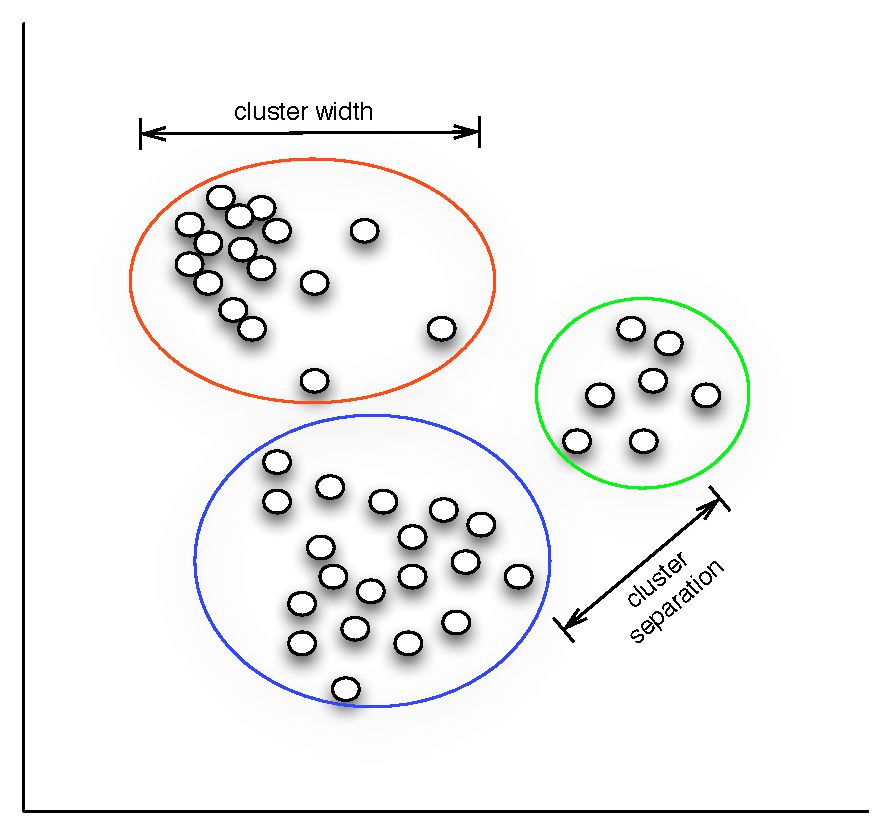
\includegraphics[width=\columnwidth]{clusterbill1}
    \caption{Clustering of bills data.}
    \label{fig:cluster.bill}
  \end{figure}

\section{Conclusions}
\label{sec:conc}
Conclusions.

\section{Future work}
\label{sec:future}
By operating as a Firefox plugin, TrackMeNot does not protect against search engines tracking time of use. As a standalone application, TrackMeNot could be run in the background, even while a user is not actively browsing. This would not only provide the same semantic search noise as the current TrackMeNot implementation, but it would serve to protect the temporal search habits of users.



\bibliographystyle{abbrv}
\bibliography{final_report}
\end{multicols}
\newpage
\begin{appendix} \label{appendix}
\section*{Appendix:}
{\tiny
\begin{verbatim}
Appendix info.
\end{verbatim}
}
\end{appendix}

\end{document}
